\begin{figure}
    \begin{center}
    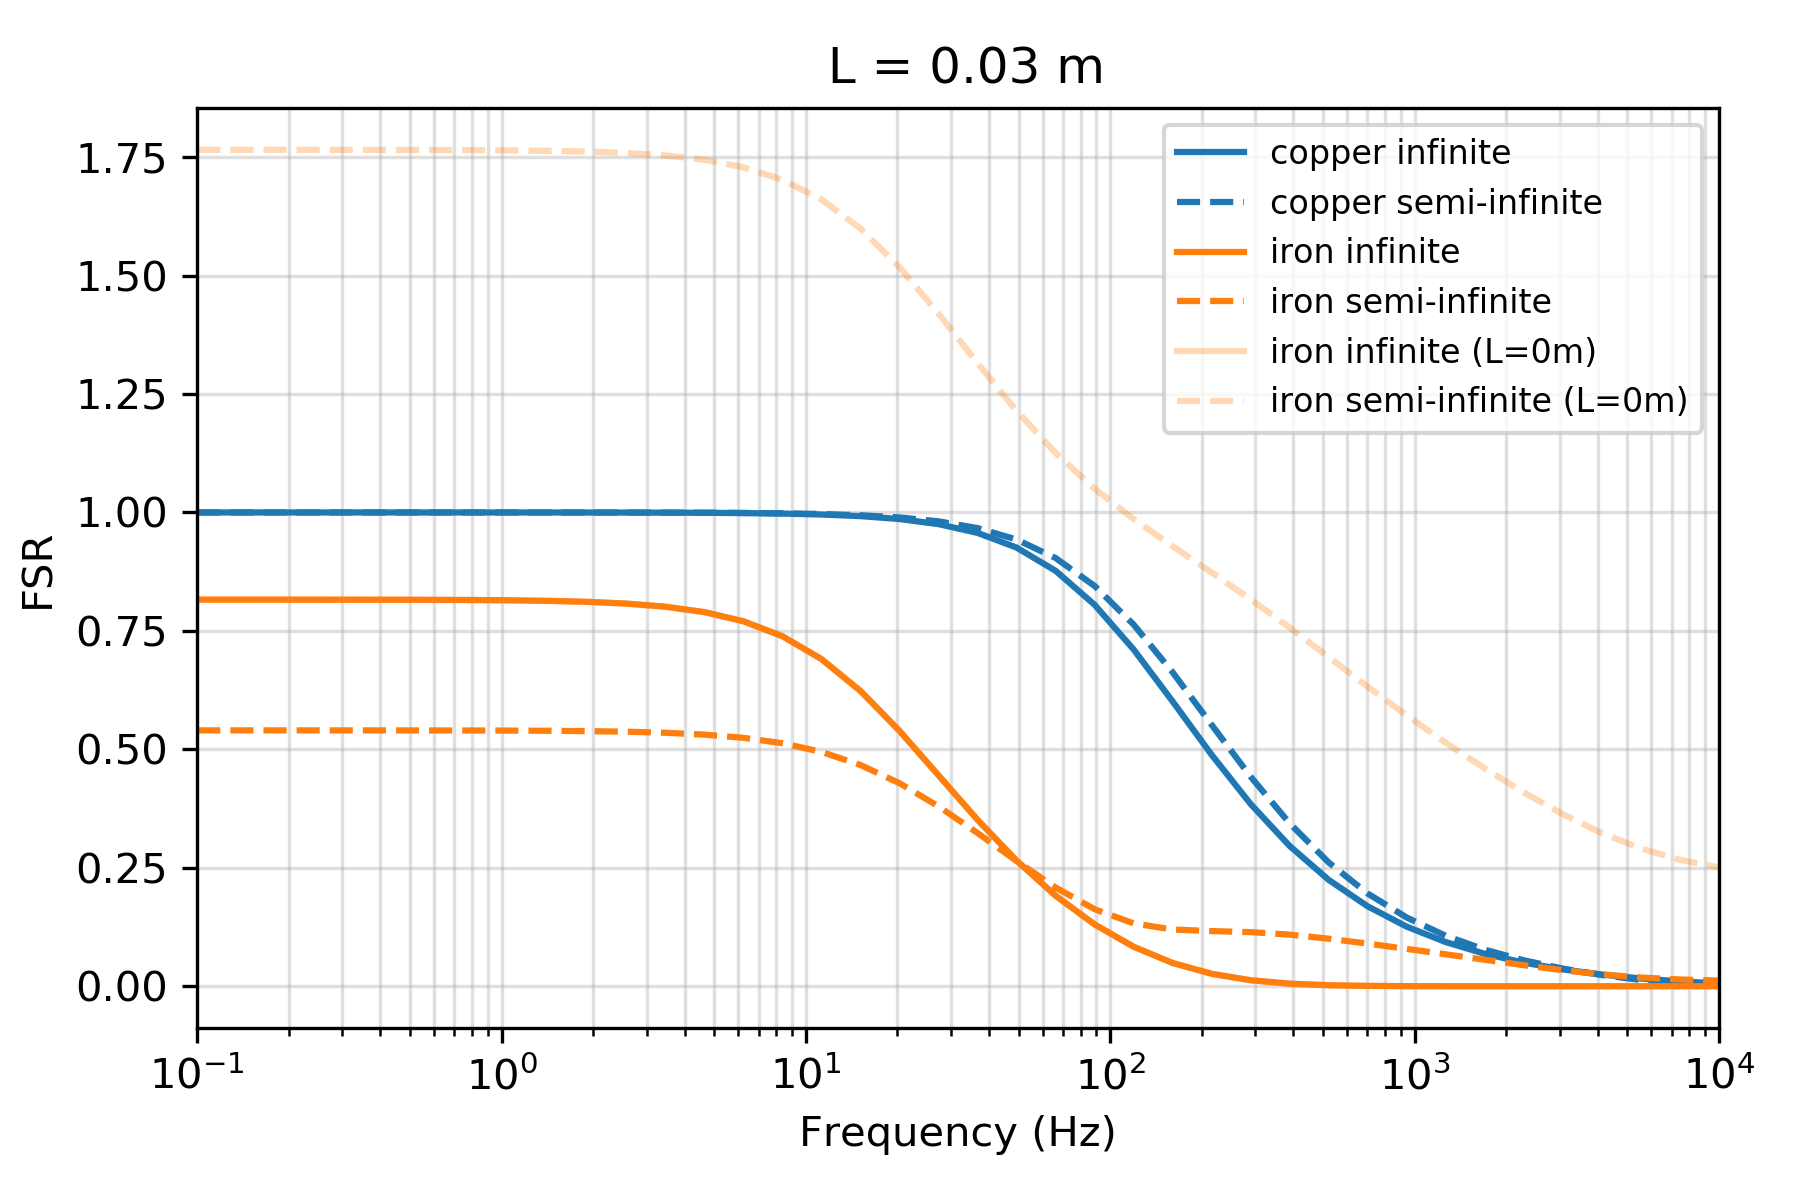
\includegraphics[width=0.6\columnwidth]{figures/Augustin3cm.png}
    \end{center}
\caption{
    Field strength ratio, FSR, for a reciever positioned 3cm beneath
    the plane of the source. For comparison, we have plotted the
    FSR for the permeable pipe when the source and reciever lie in the same
    plane (L=0.00m) with the semi-transparent orange lines.
    Note that the infinite-pipe solutions for L=0.03m and L=0.00m overlap.
}
\label{fig:Augustin3cm}
\end{figure}
